\documentclass[tikz, border=7pt]{standalone}

\usepackage[T1]{fontenc}
\usepackage[english]{babel}
\usepackage{fourier}

\usepackage{xcolor}
\definecolor{wheat}{RGB}{245,222,179}

\usepackage{standalone}

\usepackage{pgfplots}

\usepackage{tikz}
\usetikzlibrary{shapes, arrows, shadows, calc, decorations}

\usepackage{amsmath}

\tikzstyle{data}=[
  draw,
  font=\Large,
  align=center,
  minimum height=2.5em,
  drop shadow,
  rounded corners
]

\pgfplotsset{compat=1.14}

\begin{document}
	\pgfdeclarelayer{background}
    \pgfdeclarelayer{foreground}
    \pgfsetlayers{background,main,foreground}

    \begin{tikzpicture}
    	\node (residual) at (0,0) {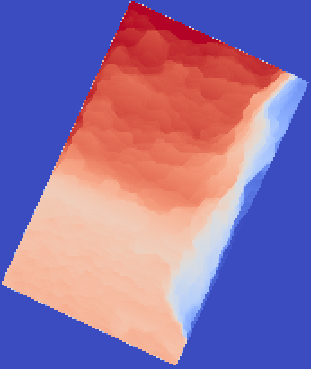
\includegraphics[height=1cm, angle=270]{images/residual}};
        \path (residual.south) + (0,-.2) node (residual_legend) {\tiny (c) Height based};
        
        \path (residual.west) + (-.8,0) node (facet_graph) {\includestandalone[mode=buildnew, height=1cm]{building_graph}};
        \path (facet_graph |- residual_legend) node (facet_graph_legend) {\tiny (b) Geometric};

        \path (facet_graph.west) + (-1,0) node (model) {\includestandalone[mode=buildnew, height=1cm]{building_model}};
        \path (model |- residual_legend) node (model_legend) {\tiny (a) Input model};
        
        \path (residual.east) + (.8,0) node (ortho_projection) {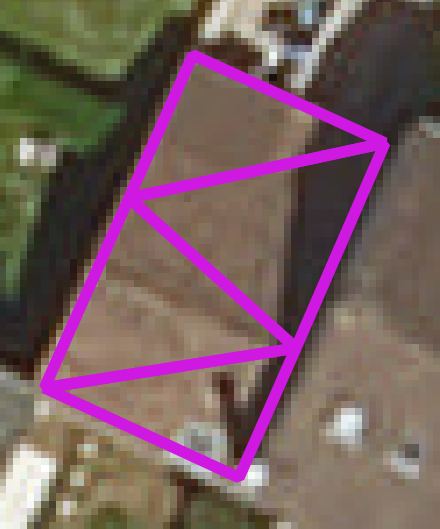
\includegraphics[height=1cm, angle=270]{images/orthoprojection}};
        \path (ortho_projection |- residual_legend) node (orthoprojection_legend) {\tiny (d) Image based};
        
        \draw[decorate, decoration={brace, amplitude=3pt}] (facet_graph.north west) -- (ortho_projection.east |- facet_graph.north) node[midway, yshift=5pt]{\tiny Features};

		\path (ortho_projection.east) + (1,0) node (errors) {\includestandalone[mode=buildnew, height=1cm]{building_errors}};
        \path (errors |- residual_legend) node (errors_legend) {\tiny (d) Erroneous building:};
        \path (errors_legend.south) + (0,-.1) node[align=left] (errors_list) {\tiny {\color{red}$\blacksquare$ Geometric error}.};
         \path (errors_list.south) node[align=left] (errors_list) {\tiny {\color{blue}$\blacksquare$ Topological error}.};
         
         \path[draw, ->, line width=1pt, rounded corners=10pt, green] (model.east) -- (facet_graph.west);
         \path[draw, ->, line width=1pt, rounded corners=10pt, green] (ortho_projection.east) -- (errors.west);
    \end{tikzpicture}
\end{document}
